% ECE4900W Communicating Engineering Solutions
% Author: Arturo Salinas-Aguayo <artjsalina5@uconn.edu>
\documentclass{beamer}
\usetheme{Warsaw}
\usecolortheme{dolphin}
\usefonttheme{professionalfonts}
\setbeamertemplate{navigation symbols}{}
\usepackage{graphicx}
\usepackage{tavox}

\title[Safe Nuclear Power]{Safe Nuclear Power: Instrumentation, Human Oversight, and Infrastructure Transition}
\subtitle{ECE 4900W – Summer 2025}
\author[Arturo Salinas]{Arturo Salinas-Aguayo}
\institute[UConn]{University of Connecticut\\College of Engineering}
\date{\today}

\graphicspath{{../../images/}}
% Bibliography
\addbibresource{references.bib}

\begin{document}

\begin{frame}
  \titlepage
  \speak{Welcome. This presentation explores the technological, ethical, and infrastructural dimensions of nuclear power in the modern world.}
\end{frame}

\begin{frame}{Outline}
  \tableofcontents[pausesections]
  \speak{Here is an overview of the major themes we will discuss today.}
\end{frame}

\section{Introduction}

\begin{frame}{Motivation}
  \speak{Nuclear energy offers unmatched energy density and reliability. Yet its history demands vigilance, ethics, and technical excellence.}
  \begin{itemize}
    \item Low emissions, high stability
    \item Risk perception shaped by major accidents
    \item Focus of this work: instrumentation, human oversight, infrastructure
  \end{itemize}
\end{frame}

\section{Instrumentation and Control}

\begin{frame}{Types of Reactors}
  \speak{Different reactor types use different coolants and designs, influencing their control strategies.}
  \begin{itemize}
    \item Pressurized Water Reactor (PWR)
    \item Boiling Water Reactor (BWR)
    \item CANDU (Heavy Water Reactor)
    \item Gas-Cooled Reactor (AGR)
  \end{itemize}
\end{frame}

\begin{frame}{Instrumentation in a PWR}
  \speak{This diagram shows how sensors monitor power, pressure, and temperature throughout a PWR.}
  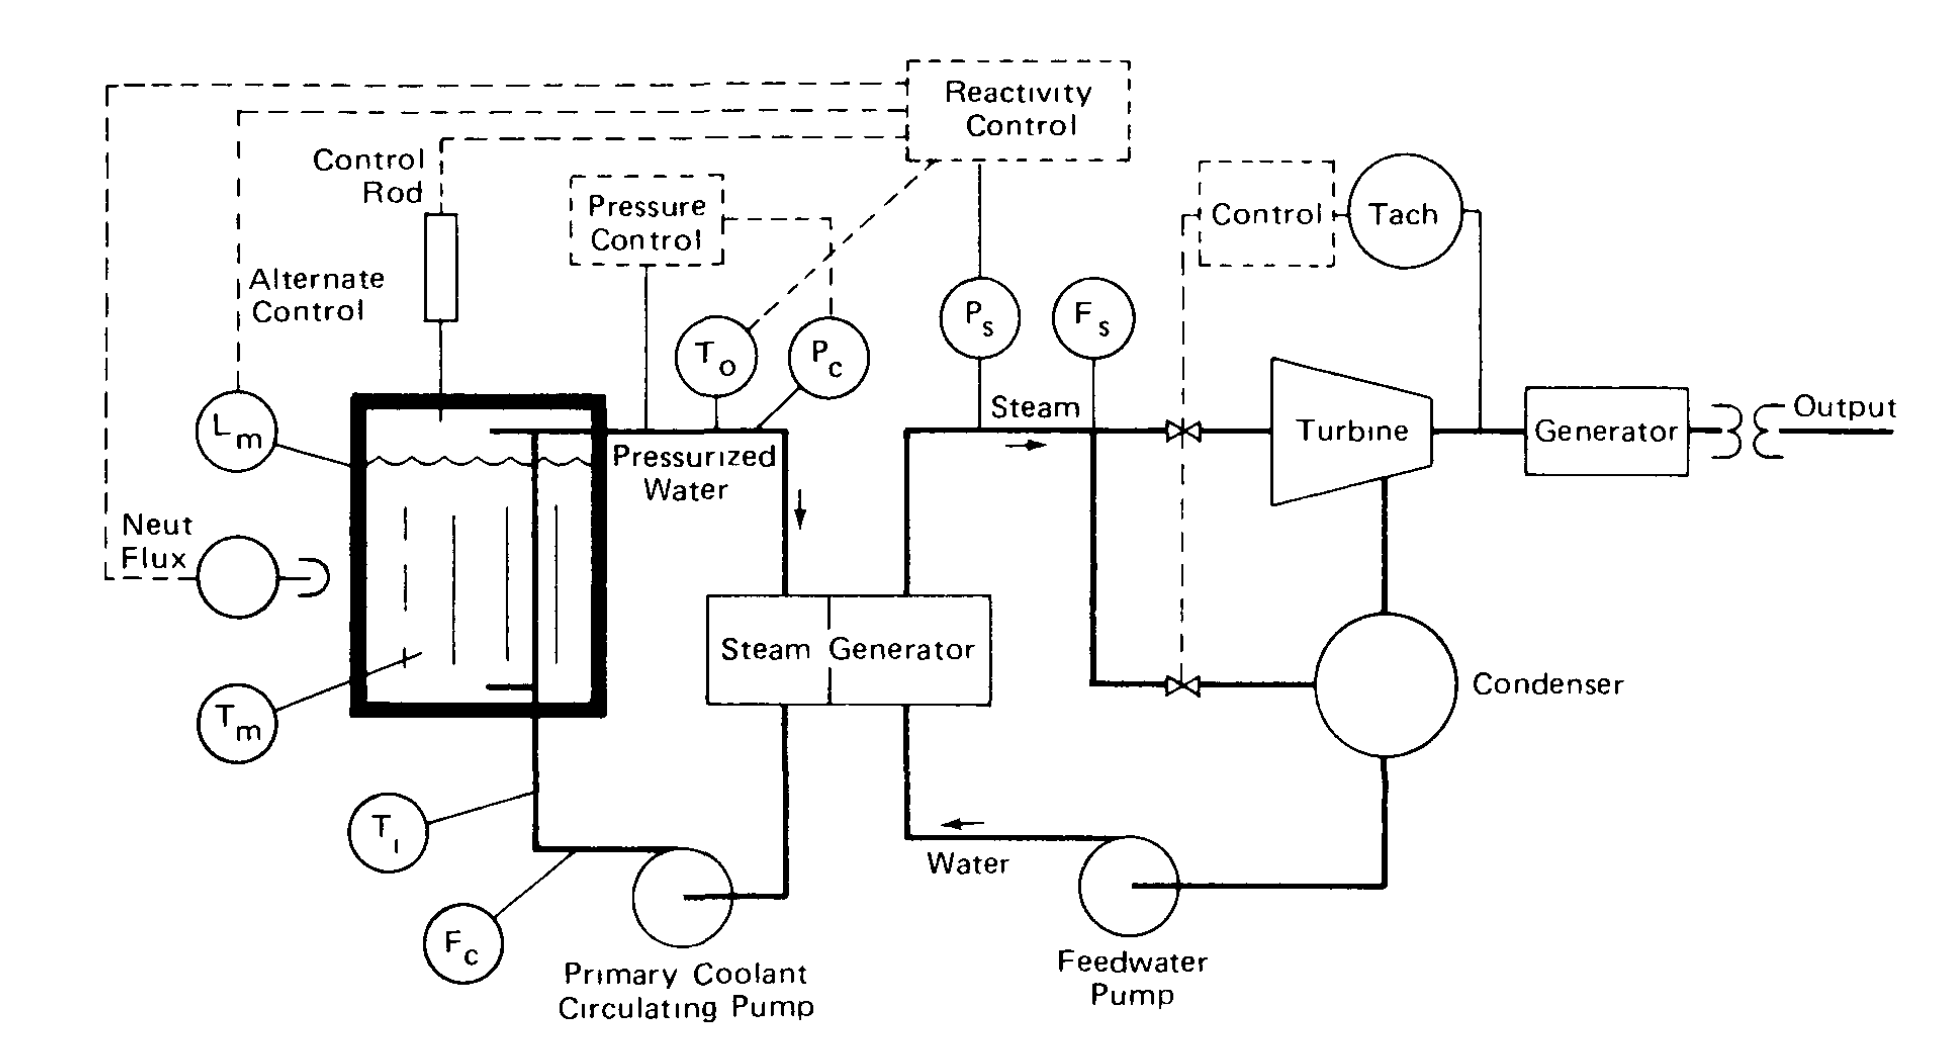
\includegraphics[width=0.85\textwidth]{images/instrumentation.png}
\end{frame}

\section{Historical Lessons}

\begin{frame}{SL-1 and Three Mile Island}
  \speak{SL-1 and Three Mile Island showed the risks of inadequate interlocks and overwhelming operator interfaces.}
  \begin{itemize}
    \item SL-1: control rod ejection, fatal steam explosion
    \item TMI: misread signals led to core exposure
    \item Both: highlight flaws in human-system integration
  \end{itemize}
\end{frame}

\begin{frame}{Chernobyl and Fukushima}
  \speak{Chernobyl and Fukushima illustrate the danger of flawed assumptions and the limits of automation.}
  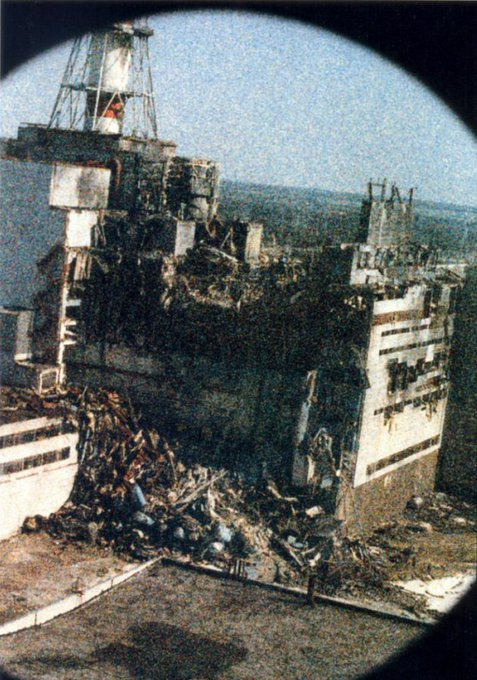
\includegraphics[width=0.75\textwidth]{images/chernobylafter.jpg}
  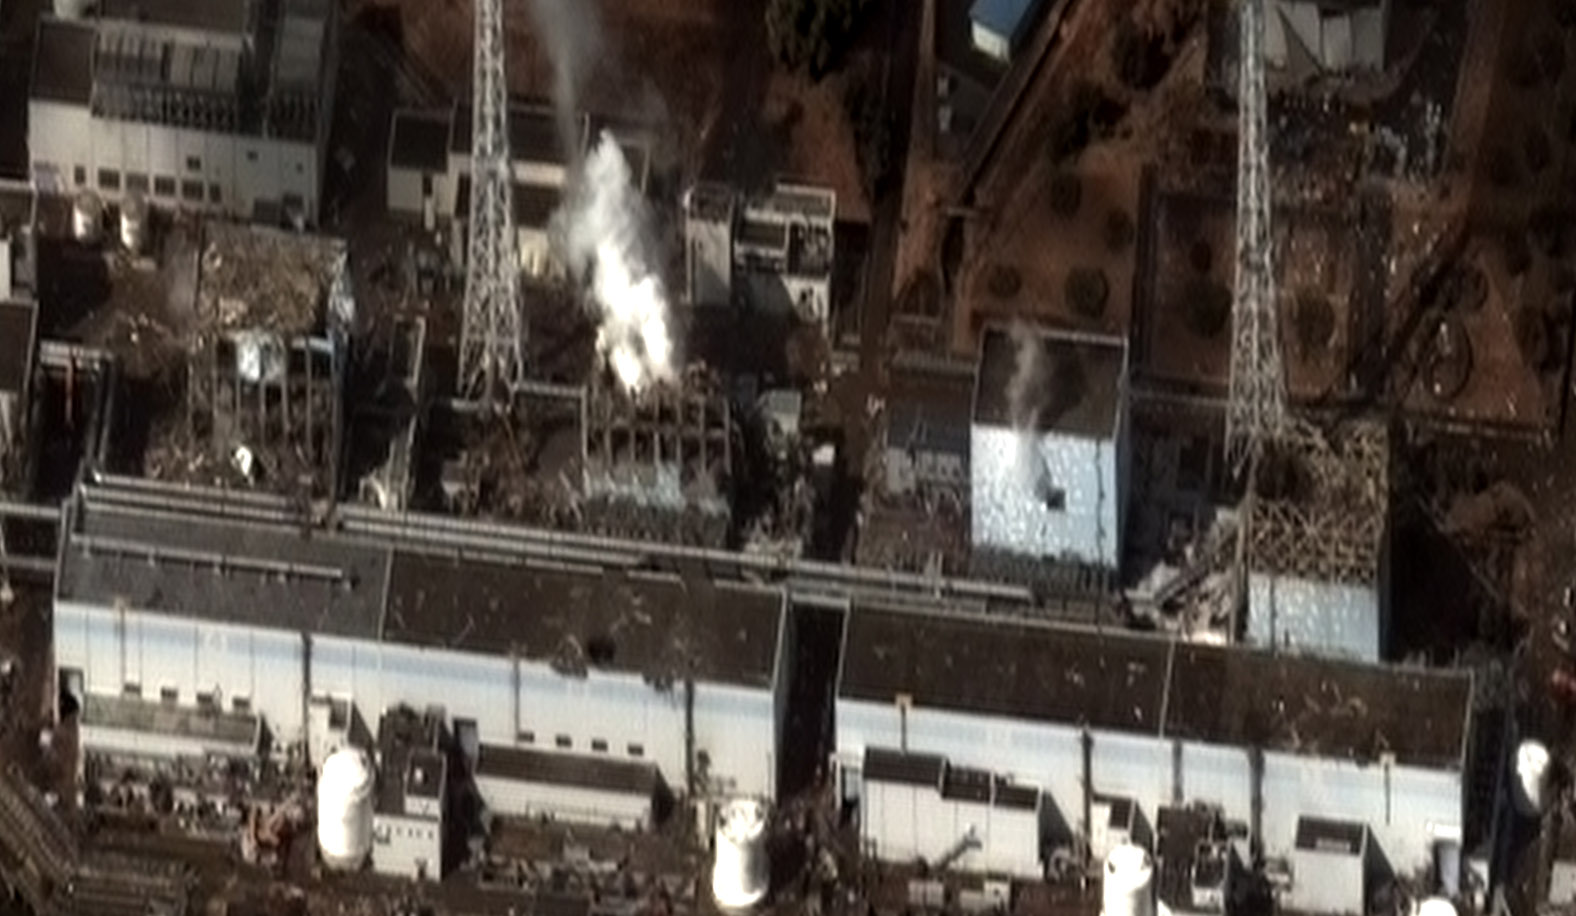
\includegraphics[width=0.75\textwidth]{images/fukushimaafter.jpg}
\end{frame}

\section{Human Factors}

\begin{frame}{Human Factors Engineering}
  \speak{Human factors engineering is vital in designing systems that support, not hinder, decision making.}
  \begin{itemize}
    \item Ergonomic control rooms
    \item Full-scope simulation
    \item Situational awareness tools
  \end{itemize}
\end{frame}

\begin{frame}{Ethics of Automation}
  \speak{Automation must be supervised. Tunnel vision and outdated assumptions can cause failure without human oversight.}
  \begin{itemize}
    \item Humans mitigate uncertainty and change
    \item Ethics demand human-in-the-loop
  \end{itemize}
\end{frame}

\section{Economic Challenges}

\begin{frame}{Waste and Infrastructure}
  \speak{The economic burden of waste management and infrastructure decline limits nuclear's future.}
  \begin{itemize}
    \item High refueling and decommissioning costs
    \item No permanent U.S. waste site
    \item Industry contraction post-Fukushima
  \end{itemize}
\end{frame}

\begin{frame}{Hopeful Developments}
  \speak{New efforts like Vogtle and SMRs show a path forward. Nuclear remains vital for base-load generation.}
  \begin{itemize}
    \item Vogtle Unit 4 completed
    \item Passive safety designs
    \item Small Modular Reactors
  \end{itemize}
\end{frame}

\section{Conclusion}

\begin{frame}{Final Thoughts}
  \speak{With humility and innovation, nuclear energy can be safe, ethical, and essential in the fight against climate change.}
  \begin{itemize}
    \item Ethics + engineering = resilient systems
    \item Human vigilance must never be replaced
    \item The atom, split with care, still holds promise
  \end{itemize}
\end{frame}

\end{document}
